\documentclass{article}
\usepackage[T1]{fontenc}
\usepackage{amssymb, amsmath, graphicx, subfigure, multicol, algorithm, algpseudocode, listings, hyperref, tikz, pgfplots}
\hypersetup{
    colorlinks=true,
    linkcolor=blue,
    filecolor=magenta,
    urlcolor=cyan,
}

\setlength{\oddsidemargin}{.25in}
\setlength{\evensidemargin}{.25in}
\setlength{\textwidth}{6in}
\setlength{\topmargin}{-0.4in}
\setlength{\textheight}{8.5in}

\newcommand{\heading}[6]{
  \renewcommand{\thepage}{#1-\arabic{page}}
  \noindent
  \begin{center}
  \framebox{
    \vbox{
      \hbox to 5.78in { \textbf{#2} \hfill #3 }
      \vspace{4mm}
      \hbox to 5.78in { {\Large \hfill #6  \hfill} }
      \vspace{2mm}
      \hbox to 5.78in { \textit{Notes By: #4 \hfill #5} }
    }
  }
  \end{center}
  \vspace*{4mm}
}

\newtheorem{theorem}{Theorem}
\newtheorem{definition}[theorem]{Definition}
\newtheorem{remark}[theorem]{Remark}
\newtheorem{lemma}[theorem]{Lemma}
\newtheorem{corollary}[theorem]{Corollary}
\newtheorem{proposition}[theorem]{Proposition}
\newtheorem{claim}[theorem]{Claim}
\newtheorem{observation}[theorem]{Observation}
\newtheorem{fact}[theorem]{Fact}
\newtheorem{assumption}[theorem]{Assumption}

\newenvironment{proof}{\noindent{\bf Proof:} \hspace*{1mm}}{
	\hspace*{\fill} $\Box$ }
\newenvironment{proof_of}[1]{\noindent {\bf Proof of #1:}
	\hspace*{1mm}}{\hspace*{\fill} $\Box$ }
\newenvironment{proof_claim}{\begin{quotation} \noindent}{
	\hspace*{\fill} $\diamond$ \end{quotation}}

\newcommand{\problemset}[3]{\heading{#1}{CS61B: Data Structures}{#2}{Alex Kazorian}{#3}{Section 4: Asymptotics}}



%%%%%%%%%%%%%%%%%%%%%%%%%%%%%%%%%%%%%%%%%%%%%%%%%%%%%%%%%%%%%%%%%%%%%%%%%%%%%%%
% PLEASE MODIFY THESE FIELDS AS APPROPRIATE
\newcommand{\problemsetnum}{1}          % problem set number
\newcommand{\duedate}{\today}
\newcommand{\studentname}{} % problem set deadline
% PUT HERE ANY PACKAGES, MACROS, etc., ADDED BY YOU
%
%%%%%%%%%%%%%%%%%%%%%%%%%%%%%%%%%%%%%%%%%%%%%%%%%%%%%%%%%%%%%%%%%%%%%%%%%%%%%%%
\usepackage{color}

%New colors defined below
\definecolor{codegreen}{rgb}{0,0.6,0}
\definecolor{codered}{RGB}{204,0,0}
\definecolor{codeblue}{RGB}{0,128,255}
\definecolor{backcolour}{rgb}{0.95,0.95,0.92}

%Code listing style named "mystyle"
\lstdefinestyle{mystyle}{
  commentstyle=\color{codegreen},
  keywordstyle=\color{codeblue},
  stringstyle=\color{codegreen},
  basicstyle=\ttfamily,
  breakatwhitespace=false,
  breaklines=true,
  captionpos=b,
  keepspaces=false,
  showspaces=false,
  showstringspaces=false,
  showtabs=false,
  tabsize=2
}

\lstset{style=mystyle}
%%%%%%%%%%%%%%%%%%%%%%%%%%%%%%%%%%%%%%%%%%%%%%%%%%%%%%%%%%%%%%%%%%%%%%%%%%%%%%%
\begin{document}
\problemset{\problemsetnum}{\duedate}{\studentname}

\section*{Overview}
Asymptotics is the study of program behavior over large input sizes. Ideally, our programs should be fast and we want to be able to analyze a given program to make sure that it is as efficient as can be. Here by efficiency, we mean the runtime of the program. There are several things necessary to discuss with regards to asymptotic analysis. This includes Big-$\Omega$, Big-$\Theta$, and Big-$O$ bounds as well as case-by-case analyses.

\section{Functions and Programs}
The functions and programs we write can be thought of as functions in the mathematical sense. They both take in an input and spit out some output. Like mathematical functions, our program runtimes grow at varying rates depending on the amount of work done. Consider the following functions that model the \texttt{runtime} of two programs (i.e the output of the function is how long it takes the program to execute):
\begin{center}
\begin{tikzpicture}
\begin{axis}[
    axis lines = left,
    xlabel = $n$,
    ylabel = {run time},
]
%Below the red parabola is defined
\addplot [
    domain=0:1,
    samples=100,
    color=red,
]
{x};
\addlegendentry{$f(n) = n$}
%Here the blue parabloa is defined
\addplot [
    domain=0:1,
    samples=100,
    color=blue,
    ]
    {x^2};
\addlegendentry{$f(n)' = n^2$}

\end{axis}
\end{tikzpicture}
\end{center}
Looking at the above plots of the functions, it seems that $f(n)'$ has smaller outputs and therefore a faster runtime when compared to $f(n)$ for the given domain; however, the domain is from $n \in [0, 1]$. In asymptotic analysis we care about the \texttt{trend} of a program's runtime as the input grows. So before we take a look at another plot with a larger domain size, let us take a look at these two functions through a more mathematical lense. While not necessary for this course, it is interesting to take the limit of these two functions as the input size grows:
\begin{align}
    \lim_{n\to\infty} \frac{f(n)}{f(n)'} &= \lim_{n\to\infty} \frac{n}{n^2} \\
                                         &= \lim_{n\to\infty} \frac{1}{n} = 0.
\end{align}
Note to get from line $(1)$ to $(2)$, we invoked L'Hospitals rule and compared the limit of the derivates of the two functions. Here it is clear that $f(n)'$ dominates $f(n)$ and therefore has a slower runtime as the input size grows. Now, lets take a bit of a step back and plot the functions to show that our intuition here was correct.

\begin{center}
\begin{tikzpicture}
\begin{axis}[
    axis lines = left,
    xlabel = $n$,
    ylabel = {run time},
]
%Below the red parabola is defined
\addplot [
    domain=0:100,
    samples=100,
    color=red,
]
{x};
\addlegendentry{$f(n) = n$}
%Here the blue parabloa is defined
\addplot [
    domain=0:100,
    samples=100,
    color=blue,
    ]
    {x^2};
\addlegendentry{$f(n)' = n^2$}

\end{axis}
\end{tikzpicture}
\end{center}
Indeed we were correct!
\subsection{Some Rules}
There are rules we have put in place to simplify asymptotic analysis. The main one being that we drop constant factors and only consider the \texttt{dominating} terms when comparing functions of the runtime of our programs. For the rest of this discussion, let $f(n) = 4n + 10000$ and $g(n) = n^3 - n^2 - n - 10000$. By dropping the constants here, we mean we should only consider $f(n)' = n$ and $g(n) = n^3 - n^2 - n$. We also said that we only consider the dominating terms in our function of runtimes and so we should have $f(n)'' = n$ and $g(n)'' = n^3$. But why is this the case?
\subsubsection{Leave the Smaller Terms Behind!}
To see why constant factors and the smaller terms are unnecessary, we take the limit of $\frac{f(n)}{f(n)'}$ as $n$ approaches infinity:
\begin{align}
    \lim_{n\to\infty} \frac{f(n)}{f(n)'} &= \lim_{n\to\infty} \frac{4n + 10000}{n^3 - n^2 - n - 10000} \\
                                            &= \lim_{n\to\infty} \frac{4}{n^2 - n} = 0
\end{align}
We again invoked L'Hospital's rule and were able to see that $g(n)$ as a function of run time grows faster than $f(n)$. Note that if we were to invoke L'Hospital's rule once more, then we would have been left with:
        $$\lim_{n\to\infty} \frac{0}{n}$$

\newpage

Here it is clear that when taking the limit of the ratio of the two functions, the only thing that matters is the dominating terms. Why? Because all that was left in the end was $n$ in the denominator which was the result of taking the second derivative of the two functions. For this reason, we can drop constant factors and only keep the largest terms in our functions of program runtime. To justify this further, let us plot this out!
\begin{center}
\begin{tikzpicture}
\begin{axis}[
    axis lines = left,
    xlabel = $n$,
    ylabel = {run time},
]
%Below the red parabola is defined
\addplot [
    domain=0:100,
    samples=100,
    color=red,
]
{4 * x + 10000};
\addlegendentry{$f(n) = 4n + 10000$}
%Here the blue parabloa is defined
\addplot [
    domain=0:100,
    samples=100,
    color=blue,
    ]
    {x^3 - x^2 - x - 10000};
\addlegendentry{$g(n) = n^3 - n^2 - n - 10000$}
\addplot [
    domain=0:100,
    samples=100,
    color=red,
]
{x};
\addlegendentry{$f(n)' = n$}
\addplot [
    domain=0:100,
    samples=100,
    color=blue
]
{x^3};
\addlegendentry{$g(n)' = n^3$}
\end{axis}
\end{tikzpicture}
\end{center}
With this plot it becomes clear that $f(n)$ behaves like $f(n)' = n$ and $g(n)$ behaves like $g(n)' = n^3$. We capture this notion by claiming $f(n)$ and $g(n)$ are proportional to $f(n)'$ and $g(n)'$ respectively. Here we introduce some notation:
\begin{align*}
    f(n) &\in \Theta(n) \\
    g(n) &\in \Theta(n^3)
\end{align*}
The above can be parsed and understood in a more formal english statement as $f(n)$ is proportional to the family of functions in $n$. A similar statement can be made for $g(n)$. What is it?

\section{Bounds}
Previously, we introduced the $\Theta$ bound to state that a function of a program's runtime is proportional to (i.e behaves \texttt{exactly} like) some function family. To clarify, you can think of a function family as the set of all functions with the same dominating term. The family of functions in $n$ is therefore the set of all functions with the dominating term of $n$. We now introduce two new bounds to help us capture some more behaviors of runtimes.
\subsection{Big-$O$}


% Put bibliography here (if any).
% Example:
%
%\begin{thebibliography}{99}
%
% \bibitem[CLRS]{CLRS}
% Thomas H. Cormen, Charles E. Leiserson, Ronald L. Rivest, and Clifford Stein,
% \emph{Introduction to Algorithms}, Second Edition.
% MIT Press and McGraw-Hill, 2001.
%
%\end{thebibliography}

\end{document}
%%%%%%%%%%%%%%%%%%%%%%%%%%%%%%%%%%%%%%%%%%%%%%%%%%%%%%%%%%%%%%%%%%%%%%%%%%%%%%%
